\section{Parallel Computing, the GPU Architecture and OpenCL}

As CPU clock speeds started to reach an upper bound in terms of raw
clock speed in about 2004~\cite{clockspeed}, processor manufacturers
started to look for new ways to increase the speed of computation in
computers. It was quickly shown that parallelization and parallel
architectures could offer great speedups in terms of performance, even
though the raw clock speed was limited. The idea is simple: use two or
more cores in parallel to work on different aspects of a problem and
merge the results in an effective manner.

As an example, suppose that we want to increment all elements in an
array of $n$ integers by one. Doing this using a traditional CPU,
would require $n$ sequential operations on the array. However, if two
traditional CPUs could somehow share the memory between them, then one
of the CPUs could process one half of the array, while the other CPU
processes the other half at the same time. We still require $n$
operations on the array, but it only takes half the time. Naturally,
while that may not be the general case, in this particular example, we
could keep on adding processing for even greater performance gains
(limited by the total size of the array, memory transfer speed and
delay, as well as management overhead).

Parallelization can be achieved in many ways. Here we will discuss
some of the most common parallel architectures in use today.

\subsection{Parallel architectures}

\emph{Grid computing systems}, where computation takes places across
multiple independent administrative domains, offer parallel
computation on an immense scale. Grids, as they are also called, are
comprised of many different devices owned by separate entities who
pool their resources together. A famous example of grid computing is
the SETI@home project~\cite{seti}, where hundreds of thousands of
people around the globe connect over the internet to volunteer their
computer resources towards the search for extraterrestrial life. The
project has since spawned the BOINC~\cite{boinc-other} grid-computing
framework, which is used to research things like protein folding using
the same techniques. These systems offer massive computational power,
but with very low speed of communication, as well as the need to have
a central server delegate sub-tasks to the individual participants in
the grid. As a result of the low speed of transfer, the sub-tasks must
be relatively independent and must be computationally time consuming
compared to their data-size for grids to be efficient.

\emph{MMP (Massively Parallel Processor) systems}, commonly associated
with supercomputers, frequently take up entire storage
facilities~\footnote{At the time of this writing, the fastest
  supercomputer in the world, according to TOP500~\cite{top500}, is
  the Titan Cray XK7, which takes up over 400
  m².~\cite{supercomputer-size}.}, and are composed of thousands of
processors connected with highly specialized hardware that have been
constructed specifically for the purpose of the supercomputer. They
typically offer very high computational power and much faster
communication between processors than grids, but at an enormous
cost~\footnote{According to Wikipedia, The Titan cost \$97
  million.}. These machines are typically owned by government
institutions and agencies or big corporations, and are mostly used for
research.

\emph{Cluster server systems}, are composed of multiple general
purpose computers that share computational resources and data across a
specialized or conventional network. Typically used for servers in
businesses, they are not quite as expensive as supercomputers, but
provide a significant boost in power compared to traditional servers,
as well as the ability to provide redundancy and fail-over services.

\emph{Symmetric multiprocessing (SMP) systems}, is an architecture
with multiple identical processors connected as a single
unit. Examples of these include motherboards with multiple CPU
sockets, allowing for more than one physical CPU.

\emph{Multi-core processors} is an example of a symmetric
multi-processing system, which consist of a single chip with more than
one computing core. Many modern CPUs contain more than a single core,
the 3rd generation Intel Core i7 processor, for example, contains 4
cores~\cite{intelcorei7}, but multi-core processors are commonly
associated with video cards. Video cards include one or more
\emph{Graphical Processing Units (GPU)}, which is a multi-core
processor specifically designed for certain parallel kinds of
operations pertaining to graphics processing. Originally designed and
sold to consumers to enhance 3-D graphics in video games, because of
their parallel architecture, GPUs have since found many other
applications, giving rise to the (quite contradictory) term
\emph{General Purpose Graphical Processing Unit (GPGPU)}. It is this
kind of parallel architecture, and specifically GPUs, that we wish to
take advantage of with SmlCL.

\subsection{Graphical Processing Units}

Modern GPUs include hundreds or thousands of cores that all can be
used in parallel to effectively perform such things as matrix
operations and operations on large arrays; when it comes to these
kinds of operations GPUs offer huge speed gains compared to
traditional CPUs, at an affordable price.

GPU architectures, such as NVIDIAs Kepler GK110, typically consist of
a large number of cores grouped in a smaller number of groups. On top
of an amount of shared memory between all groups, each group has its
own memory that all cores in the group can uniformly access.

\begin{figure}
  \centering
  \caption{Diagram of NVIDIAs Kepler GK110 architecture}
  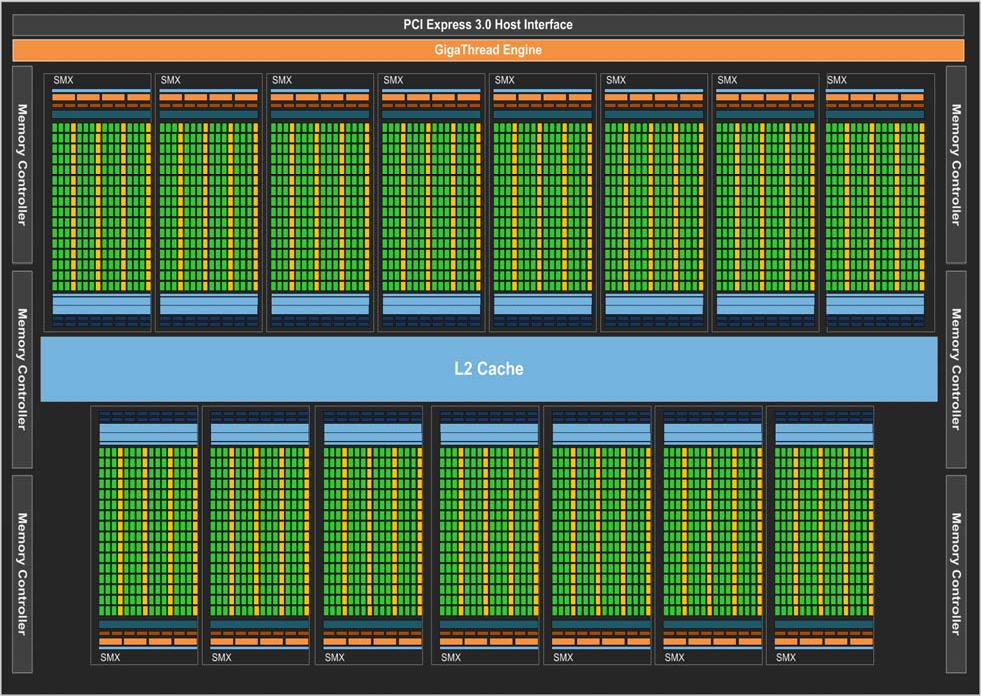
\includegraphics[width=1\textwidth]{figures/kepler110.png}
  \label{kepler}
\end{figure}

As an example, the Kepler GK110 is equipped with 15 groups of cores,
called \emph{Streaming Multiprocessors (SMX)}, each with 192
single-precision cores, and 64 double-precision cores and several
other cores for more specific operations~\cite{kepler}. Each streaming
multiprocessor has 64 KB of memory that is shared between its cores,
in addition to 1536 KB memory that is shared between all of the
streaming multiprocessors.

In order to take advantage of all this parallel processing power in an
efficient manner, special care must be taken when programming for the
GPU. We have to divide the work into parts, distribute them across
groups and cores, make sure that cores do not overwrite the work of
each other, synchronize results and so on, while also taking into
account that transferring data from the CPU to the GPU is likely to
take a long time. Luckily, frameworks, such as \emph{OpenCL}, can help
us with these tasks~\footnote{CUDA is another popular framework,
  specifically for programming NVIDIA GPUs. While Smlcl will focus on
  GPU programming, we also want to allow other GPUs than NVIDIAs,
  which is why we've chosen to work with OpenCL}.

\subsection{OpenCL}

Originally created by the non-profit technology consortium Khronos
Group~\cite{khronos}, and since embraced by numerous hardware and
software companies, including AMD and NVIDIA, the two biggest
manufacturers of GPUs, OpenCL\cite{opencl} is ``a framework suited for
parallel programming of heterogeneous
systems''~\cite[p.~35]{clbook}. With it, you can write programs that
can run on both CPUs and GPUs, as well as Digital Signal
Processors and other kinds of processors supporting the framework,
allowing us to take advantage of many different architectures using
the same code.

In OpenCL, programs are made up of \emph{kernels}, which are written
in a C-like language, and some host code which makes calls to the
OpenCL API in order to execute said kernels. Each kernel takes a set
of arguments, performs some kind of computation, and modifies one or
more of the arguments to include the result of the computation (in
OpenCL, kernels cannot return values, therefore results are returned
to the caller via in-memory data-structures). \emph{Work groups} are
made up of a number of kernels, and arguments to kernels can be either
global (all kernels access the same memory), local (only kernels in
the same work group can access the same memory) or private (no other
kernel can access this memory). Each kernel also has a unique global
ID, a work group ID, and a unique ID within it's work group.

The host code, typically written in C or C++, uses the
OpenCL API to set up the OpenCL environment for a specific device,
compile and build the kernel code, transfer data to buffers on the
device, execute the kernels and read the results back from the
buffers. Appendix \ref{app:vectoradd}, shows the code required to
calculate the addition of two vectors. In short, the steps required
are:

\begin{enumerate}
  \item Get the \texttt{cl\_platform\_id} for the platform that we
    want to work with.
  \item Get the \texttt{cl\_device\_id} the device that we want to
    work with.
  \item Create a \texttt{cl\_context} for the device and platform
    chosen. \emph{Contexts} are used by the OpenCL runtime to manage
    command-queues, memory, program, and kernel objects, as well as
    for executing kernels.
  \item Create a \texttt{cl\_command\_queue} using the context
    created. When a command is to be executed on the device, it is put
    in the command queue, from whence the OpenCL runtime will
    execute it in order.
  \item Create a \texttt{cl\_program} from source code using the
    context obtained above. A \emph{program} is a collection of
    kernels, which may also contain auxiliary functions and constant
    data.
  \item Compile and link (called building) the program obtained in the
    previous step.
  \item Create a \texttt{cl\_kernel} from one of the kernels in a
    given program. A \emph{kernel} is the bit of code that is to be
    executed on the device.
  \item Create appropriate buffers (\texttt{cl\_mem} objects) for
    input and output.
  \item Write input data to the input buffers.
  \item Set arguments for the kernel created above. These can be input
    buffers, or scalars like an \texttt{int}.
  \item Put the kernel in the command-queue to execute it.
  \item Read the contents of the output buffer(s).
\end{enumerate}

As it can be seen, even executing a rather simple computation like a
vector addition, takes many steps, and simply because of the
complexity of the process, there is a high risk that the
programmer unwillingly introduces errors when writing the code. In
addition, OpenCL provides little to no feedback on what goes wrong in
case there is an error in your kernel, or how you have executed it.

This motivates us to try and create a simpler and safer interface,
that takes some of the strain off of the programmer.
